\section{Natural Sounding Schroeder Reverberation}
\label{sec:shroeder1}

La base da cui partiamo per la realizzazione del riverbero algoritmico sono gli
studi fatti da \ms~ riportati nel suo articolo
\emph{Natural Sounding Artificial Reverberation} pubblicato nel 1962 in seguito
agli esperimenti condotti a Murray Hill, presso i Bell Laboratories.

Manfred Robert Schroeder è stato un fisico tedesco conosciuto per i suoi studi
su acustica, telecomunicazioni e computer grafica. Nasce nel 1926, ad Ahlen in
Germania e già da giovane mostra interesse nell’elettronica e nelle
telecomunicazioni. Dopo un periodo di interruzione dallo studio a causa del suo
reclutamento durante la Seconda Guerra mondiale, Manfred conclude i suoi studi
sotto la tutela del prof Erwin Meyer, un’ autoritá nel mondo dell’acustica.
In seguito alla sua laurea, il suo lavoro è stato lodato dall’amministrazione
dei Bell Laboratories, i quali gli hanno offerto un impiego nella divisione di
ricerca a Murray Hill, New Jersey. Da lì in poi ha proseguito le sue ricerche
spaziando dalle telecomunicazioni all’acustica conseguendo numerosi
riconoscimenti in tutto il mondo.

Il sopracitato laboratorio Bell Labs è inoltre importante da citare in quanto,
oltre ad essere un’ istituzione nel campo delle telecomunicazioni, è un
eccezionale esempio di collaborazione e progresso. Il laboratorio era un
apparato di Bell System, una società telefonica che ha operato in America
fornendo servizi a livello nazionale. Lo scopo del laboratorio, dunque, era
quello di fornire nuove tecnologie all’avanguardia nel campo delle
telecomunicazioni. Da ciò si può facilmente intuire innanzitutto il grande
capitale e le tecnologie messe a disposizione dei ricercatori, tra cui
Schroeder, e dell’ambiente ricco di menti portate all’innovazione tecnologica.

%\subsection{Analisi}

Come detto, partiró dall’analisi fatta da Schroeder per la progettazione del
riverbero. In quel periodo, parliamo del 1962, gli studi e le tecnologie in
grado di sintetizzare un riverbero erano acerbe. Le tecniche più diffuse
all’epoca, le quali partivano delay creati su nastro magnetico, disco o molle,
non producevano un effetto fedele al riverbero naturale per 2 aspetti principali:

\begin{itemize}
\item La loro risposta, sia in frequenza che in ampiezza, non era piatta,
      comportando una “colorazione” nel risultato, soprattutto se solo una
      piccola parte del segnale diretto veniva missato al segnale riverberato.
\item La densità degli echi non era sufficiente a creare un risultato credibile.
      La ricerca di Schroeder ci mostra che circa 1000 echi al secondo è un
      risultato accettabile per un riverbero sintetico. Consideriamo che in un
      ambiente reale le riflessioni sono infinite, ma questo sarebbe un risultato
      quasi impossibile da raggiungere
\end{itemize}

Nel suo articolo \ms~ mostra il suo approccio alla risoluzione per le
problematiche sopracitate.

In primo luogo per ovviare al primo problema è necessario creare una linea di
ritardo con feedback che abbia una risposta piatta in ampiezza e frequenza.
Utilizzando lo schema proposto da schroeder, abbiamo un dispositivo
(informatico, in questo caso) incaricato di restituire un singolo eco, dopo un
ritardo temporale ($t$)

\begin{figure}[htp]
\centering
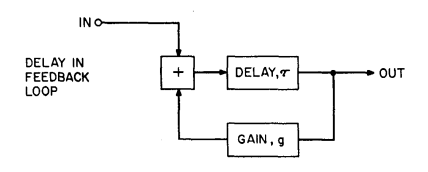
\includegraphics[width=0.80\textwidth]{dfl}
\caption{Delay all'interno di un feedback}
\label{fig:dfl}
\end{figure}

Dato che l'obiettivo è quello di produrre un elevato numero di echi a partire
da un numero contenuto di oggetti, inseriamo dunque la linea di ritardo in un
feedback avente come moltiplicatore $(g) < 1$.

Il risultato sarà un segnale che decade di $g$ volte ad ogni ciclo.

\begin{figure}[htp]
\centering
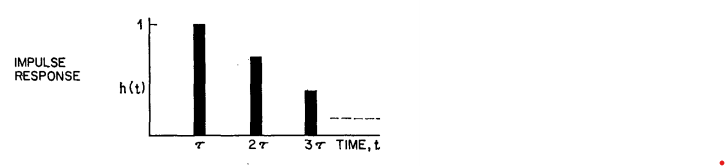
\includegraphics[width=0.80\textwidth]{dflir}
\caption{risposta in ampiezza}
\label{fig:dflir}
\end{figure}

La sua risposta in frequenza invece, presenta in modo periodico picchi e valli
sullo spettro, aventi come valori rispettivamente $(1+g)$ e $(1-g)$. L’autore,
data la somiglianza ad un pettine, rinomina il ciclo sopra descritto
\emph{Comb Filter}, e così mi riferirò al medesimo d’ora in avanti.

\begin{figure}[htp]
\centering
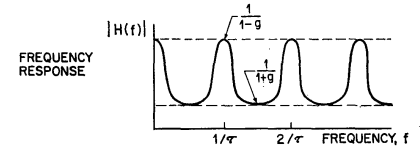
\includegraphics[width=0.80\textwidth]{dflspectrum}
\caption{rispsota in frequenza}
\label{fig:dflspectrum}
\end{figure}

Questo comportamento del filtro comporta però una certa non esattezza in
termini di spettro che Schroeder cerca di evitare, raffinando l’algoritmo
tramite successive integrazioni.
La soluzione proposta dall’autore e Logan è il missaggio del suono diretto
moltiplicato per $(-g)$ e il suono riverberato moltiplicato per $(1-g^2)$.
Questo comporta una risposta piatta per tutte le frequenze. Il filtro
risultante, chiamato \emph{All Pass Filter}, è descritto secondo il seguente
schema e per le successive integrazioni, viene utilizzato come unità
riverberante di base.

\begin{figure}[htp]
\centering
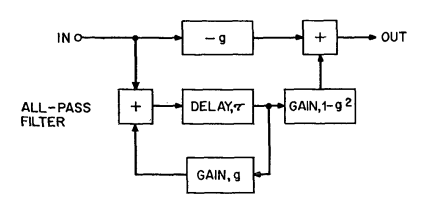
\includegraphics[width=0.80\textwidth]{apf}
\caption{All Pass filter di Schroeder}
\label{fig:apf}
\end{figure}

Per risolvere la problematica della densità degli echi, la soluzione di
Schroeder è quella di connettere in serie più riverberatori, in modo tale che
la densità cresca in modo frattale per ogni unità connessa. Dato che abbiamo
risolto il problema di una possibile colorazione del filtro, possiamo non
preoccuparci che questo avvenga per una connessione in serie.

\begin{figure}[htp]
\centering
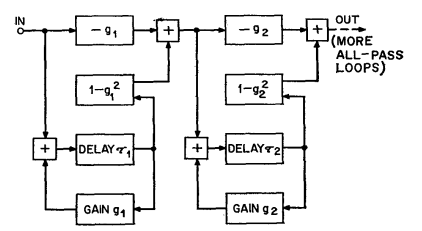
\includegraphics[width=%
0.50\textwidth]{apfseq}
\caption{sequenza di 5 All Pass}
\label{fig:apfseq}
\end{figure}

La densità che si cerca di raggiungere, ovvero quella di circa $1000$ echi al
secondo, è facilmente raggiungibile con 5 riverberatori in serie (il numero
prodotto è di circa 810). A differenza di Schroeder abbiamo a disposizione
molte più risorse, in termini di potenza di calcolo infatti possiamo
serializzare molti più riverberatori e raggiungere un numero di riflessioni
elevatissimo.

Successivamente, avendo constatato l’efficienza del riverberatore \emph{All-Pass},
Schroeder cerca di implementare alcune caratteristiche della riverberazione
naturale.

Esse sono:

\begin{itemize}
\item Missaggio del suono diretto con il suono riverberato, senza alterare la
      struttura di All Pass;
\item Inserimento di un leggero sfasamento temporale tra, appunto, il segnale
      diretto e il segnale riverberato, dato che come sappiamo, il suono diretto
      raggiunge l’ascoltatore prima delle riflessioni;
\item La dipendenza alle frequenze del tempo di riverbero;
\end{itemize}

Il segnale non riverberato restituito dalla sequenza di all-pass risulta
parecchio ininfluente, per questo Schroeder consiglia di moltiplicare per
($-g$) e sommare il segnale diretto proprio con questa serie, come illustrato
in figura \ref{fig:apfmix}.

\begin{figure}[htp]
\centering
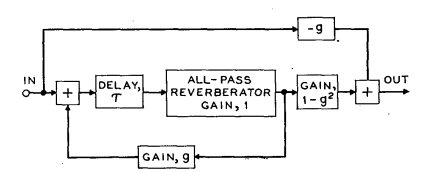
\includegraphics[width=%
0.50\textwidth]{apfmix}
\caption{sequenza di All Pass con aggiunta di segnale diretto}
\label{fig:apfmix}
\end{figure}

Il box chiamato \emph{“All-pass reverberator”} contiene, come detto, la serie di
\emph{All-Pass}, inserito all’interno di un ulteriore feedback loop.
Da notare il delay iniziale, il quale permette un ritardo rispetto al suono
diretto, rifornendo anche il secondo punto.

Un ultimo aspetto da considerare dell’articolo, è l’utilizzo combinato di filtri
\emph{Comb} e \emph{All-Pass} per ricercare, al contrario dell’obiettivo
originale, una risposta frequenziale altamente irregolare, come nel caso delle
stanze reali.
In seguito agli esperimenti condotti ai Bell Telephone Laboratories, in cui si
è scoperto che ad alte densità di riflessioni le irregolarità sono
impercettibili, si è pensato di ricostruire l’algoritmo in modo tale da ricreare
le condizioni di una stanza reale.
Lo schema è raffigurato in figura \ref{fig:comballpass}

\begin{figure}[htp]
\centering
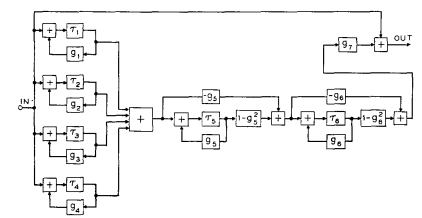
\includegraphics[width=%
0.60\textwidth]{comballpass}
\caption{Configurazione Comb-All Pass}
\label{fig:comballpass}
\end{figure}

Questa nuova configurazione conformazione prevede:
\begin{itemize}
\item Un certo numero di Filtri Comb, aventi tempi di delay incommensurabili
      oppure primi, connessi in parallelo. Questi filtri produrranno le
      cosiddette “Early reflections";
\item Un certo numero di All-Pass connessi in serie, in modo tale da
      incrementare la densità degli echi.
\item Al tutto verrà aggiunta una quantità di segnale diretto come nelle
      precedenti iterazioni.
\end{itemize}
